\documentclass[letterpaper]{article}
\usepackage[latin1]{inputenc}
\usepackage{amsmath}

\usepackage{amsfonts}
\usepackage{amssymb}
\usepackage{graphicx}
\usepackage{hyperref}
\usepackage[final]{pdfpages}
\usepackage[left=1.00in, right=1.00in, top=1.00in, bottom=1.00in]{geometry}
\author{Andrew Rosen}
\title{Research Philosophy}
\date{}
\begin{document}
\maketitle


% DO NOT USE THE WORD TOOL
% Empahsize that my research is applicable to big data problems and research
% Talk about collaberation + inter-disciplinary

\section{Executive Summary}


%I research and develop highly fault-tolerant and robust systems.


%\subsection{The Motivation for my Research}
My research area focuses on developing fault-tolerant systems because they are absolutely critical to networking and the Internet, which have become an essential part of our lives.
Fault-tolerant and robust systems are what hold a complex environment like the Internet together.
The Internet is made up of billions of devices, each the source of thousands of tiny errors every day.
The packets are dropped, the routers are poisoned, the hard drives keep crashing, someone tripped over a power cable, the software is full of bugs, and the developers meant to add security but it was adopted before we got the chance.
The Internet, by all rights, should not work, but it does because smart people decided that failure was an assumption that needed to be baked into every layer of every protocol.

Fault-tolerance is in many ways the most important part of what makes the Internet and networking work in general.
As companies grow and create larger and larger intranets and datacenters, as more people gain access to the Internet, adding billions of handheld devices that rival the power of last decade's consumer desktop, this problem is only going to get magnified.

To address these issues, my research primarily focuses on Distributed Hash Tables (DHTs), with applications towards peer-to-peer (P2P) networks, Big Data, and Distributed Computing.
DHTs are primarily used in P2P applications due to their decentralization and fault-tolerance. 
These qualities make them well suited for applications such as file-sharing, content distribution, multi-player video games, botnets, and video chat.
Their qualities also make them suited for distributed computing.



Over the course of my studies, I have worked with researchers not just in Computer Science, but Psychology, Astronomy, and Biology as well.
I have seen firsthand how fields outside Computer Science draw more and more heavily from distributed computing and big data.
My research on distributed computing over distributed hash tables has yielded a platform for solving Big Data problems that can be used to solve not just problems in Computer Science, but be used by researchers in other fields to quickly create and deploy systems for solving Big Data problems.


\section{Past and Current Work}

My past and current research focuses on using DHTs for distributed computing \cite{chordreduce} and defining a DHT at its most abstract level.
There are many different types of DHTs, but all DHTs share very important qualities.
They are \textit{scalable}, which means that each additional node in the network minimally impacts the cost of keeping the network organized.
DHTs are also highly \textit{fault-tolerant}.
Unlike many other systems, DHTs assume that nodes will be continuously entering and leaving the network.
Because of the way DHTs are organized, they can handle large scale failures, such as a power outage affecting an entire city.
The last quality of DHTs is that they are \textit{load-balancing}. 
This means the data stored in a DHT is evenly distributed among nodes in the network using a cryptographic hash function.


\subsection{Distributed Computing on a DHT}

The scalability, fault-tolerance, and load-balancing qualities of DHTs are also highly desirable qualities in a distributed computing framework.
As such, I wanted to see if it was possible to use DHTs to perform distributed computing.

ChordReduce \cite{chordreduce} was a proof of concept for using distributed hash tables for distributed computing.  
It used Chord \cite{chord}, a well-studied DHT, and exploited its various features to perform MapReduce \cite{mapreduce} tasks, a very popular method for framing distributed computing problems.

Unlike other distributed computing frameworks, we made no assumptions as to the context in which ChordReduce would be used.
ChordReduce could be used in either a large datacenter or in completely heterogeneous, peer-to-peer context.
In a heterogeneous network, we assume all the nodes represent different pieces of hardware, with differing levels of computational power and reliability.
As a result, we needed to rigorously test the fault-tolerance of the system and made an exciting discovery while doing so.

To test fault tolerance, each node essentially flipped a coin weighted in its favor, and when it lost the flip, left the network and reentered as a new node.
This simulated churn, turbulence in the network caused by the continuous entering and leaving the network.

Churn is normally a chaotic influence on the network. 
However, we found that at high levels of churn, nodes advantageously redistributed work in such a way that tests with high levels of churn performed better than tests with low levels of churn.

ChordReduce established three important ramifications.
First, we experimentally demonstrated that DHTs are capable of being used as a framework for distributed computing.
Second, DHT based distributed computing can have nodes enter the network at any time, even when a job is running, and be immediately put to work.
Finally, we discovered that while churn is normally a disruptive force, at high levels it can be helpful to the network.


\subsection{UrDHT}
I became interested in finding if there was a way of abstracting DHTs.
While there has been extensive literature defining what a DHT does, none of these rigorously define how the various pieces of a DHT can be defined.
For example, each node in a DHT has a range of keys which it is responsible for, but this range is defined differently for every DHT. 

Working with my coauthor, I found that DHTs can be cleanly mapped to Voronoi Tessellations and Delaunay Triangulations.
By treating each node as a Voronoi generator, a node's range of keys becomes its Voronoi region and edges to nearby nodes correspond with the links forming the Delaunay Triangulations.

We created a distributed greedy heuristic where each node can quickly construct its own Delaunay Triangulations and  Voronoi Tessellation \cite{dgvh}.
Our heuristic works in any geometric space where the distance is defined.

We used this to create an abstract DHT called UrDHT \cite{urdht}.
UrDHT can be used to implement the topology and functionality  of any other DHT by defining the space the DHT operates in.

UrDHT essentially acts as a ``fill-in-the-blanks'' for creating  distributed hash tables.
The novelty of UrDHT is that it makes it easy for scientists in any field to construct a DHT based application.
For computer scientists, UrDHT provides a means of rigorously comparing different architectures.

I am currently implementing the distributed computing framework on a wider variety of topologies using UrDHT and creating an autonomous load-balancing strategy for nodes within a DHT.
When I initially created ChordReduce, it used a single DHT, Chord \cite{chord}.
One of the questions we needed to examine for future research was ``did the choice of DHT topology matter, and to what extent?''
UrDHT provides an excellent means for answering this question, since  UrDHT makes it easy to construct the topology of other DHTs.


\subsection{Autonomous Load Balancing}
The larger and more interesting question I am asking is how churn can be leveraged to speed up computation.
I found in previous research that extremely high levels of random churn helped the nodes complete computation faster.
This is because the ranges of keys nodes are responsible for are unevenly sized, which means some nodes end up with more work than other nodes.

Because of the rigorous fault-tolerance we built into the system, one of these nodes going offline was only a minor inconvenience.
As the computation continues, however, more and more nodes are idle without any work.
When one of these nodes leaves the network and rejoins, it either will join in a location where it cannot acquire any additional work, or it will reenter at a location where it can.
The former case has no impact on the network's running time, whereas the latter redistributes some of the work.
This was the source of our speedup in our experiments.

If an essentially random application of churn can result in speedup, is there a strategy I can use to control this process and create a larger benefit to runtime?
I am currently examining multiple strategies that would leverage the ``benefits'' of churn.
These strategies would allow nodes to strategically and autonomously redeploy themselves to new locations when needed, which would mean workloads could be redistributed on the fly.
To address differences in computing power in a heterogeneous network, computationally stronger nodes could represent themselves as multiple nodes within the network.
This is effectively applying the Sybil attack \cite{sybil}, but in a controlled manner to the network's benefit.




%\section{Misc}
%I find great value in abstracting techniques and platforms even further, as that makes it possible to see novel applications for various technologies.  
%This can be seen in my work on Distributed Hash Tables, where I showed that DHTs can be mapped to Voronoi Tessellations and Delaunay Triangulation.
%
%
%We used this insight to create UrDHT \cite{urdht}, a generalized framework for building distributed hash tables.
%UrDHT essentially acts as a ``fill-in-the-blanks'' for creating  distributed hash tables.
%The novelty of UrDHT is that it makes it easy for scientists in any field to construct a DHT based application.
%For computer scientists, UrDHT provides a means of rigorously comparing different architectures.
%
%I believe that collaboration is vital to academic growth.
%I have worked with researchers in both Computer Science and other scientific fields, including Astronomy, Biology, and Psychology.
%
%A large part of why I do research is that I want to help people.
%When I started doing undergraduate research, I worked in the Sonification Lab at Georgia Tech.
%There, I helped PhD students implement their research in creating  non-traditional user-interfaces geared towards the visually impaired community.
%


\section{Future Research}

My work with DHTs and Voronoi Tessellations has many potential avenues for future work.
There is the direct application of the DHT computing model to various distributed computing problems, as well as further improvements on the autonomous load balancing strategies.
Over the course of developing UrDHT, I have found many potential directions in which to apply my research.


%\paragraph*{Distributed Databases}

\paragraph*{Wireless Sensor Networks Sleep Strategies} C\u{a}rbunar et al.\ \cite{carbunar2004distributed} demonstrated how Voronoi Tessellations could be used to solve the \textit{coverage-boundary} problem in wireless ad-hoc networks.
The coverage-boundary problem asks which nodes are on the physical edge of the network.
This problem  has applications such as setting sleep schedules \cite{chen2008voronoi}.
Since our greedy Voronoi heuristic is designed for a distributed environment, it is well suited for applications in WANETs. 


\paragraph*{Interdisciplinary Applications}
UrDHT has many applications for interdisciplinary research, as it makes it easy to deploy for distributed problems that occur in a wide variety of disciplines.
Monte-Carlo approximations are particularly well suited for UrDHT's computation model.

Another set of wide-ranging problems is classification.  
I can design the system to build a classification model from test samples and distribute this model to the nodes containing data to be classified.
Some examples problem this can be applied to is classifying supernovae, or evaluating random forests.


\paragraph*{Content Distribution Networks}
Content Distribution Networks (CDN) benefit heavily from the qualities of Distributed Hash Tables.
One quality provided by UrDHT is the ability to optimize routing over a desired attribute, such as latency or bandwidth.
We can use UrDHT to create a CDN which optimizes routing for bandwidth use or latency, while still maintaining the fault-tolerance and other qualities provided a DHT.


\paragraph*{Distributed DNS}
The Stop Online Piracy Act and Protect IP Act, both introduced and vigorously debated in 2011, brought attention to the fact that DNS could be fractured by filtering by the US government.
This is a consequence of DNS being centralized  and adopted before security was fully addressed.
One of my goals is to deploy a fully decentralized and distributed DNS servers using UrDHT.
A decentralized DNS service was previously considered impracticable \cite{cox2002serving}, but new technology, such as the Blockchain, have addressed a number of previous concerns.





%
%Our research would have many applications within the field of Computer Science.
%Traditional MapReduce frameworks and other distributed computing solutions are limited to being deployed solely in a datacenter \cite{hadoopAssumptions}.
%Distributed computing frameworks built with UrDHT would be able to be deployed any context, be it a data center, a P2P network, or a volunteer computing pool.
%Furthermore, the autonomous load-balancing feature would allow frameworks to automatically give nodes with more power more work.
%
%Our framework would not only be of interest to computer scientists.
%The ``plug-and-play'' nature we envision would make it easy for experts in other fields to use our framework to solve computationally intensive problems.
%Some example problems are Monte-Carlo Methods (of interest to mathematicians and economists) and machine learning (of interest to biologists).
%
%This project would allow both organizations with large amounts of computing power and average developers with  fewer resources to spend less time setting up and configuring their hardware to work together.  
%The goal is for our software to make distributed computing more of matter of ``plug-and-play,'' allowing researchers to spend less time setting up and maintaining  computing platforms.
%



\bibliography{mine,dht,mapreduce,dns,wanet}
\bibliographystyle{IEEEtran}
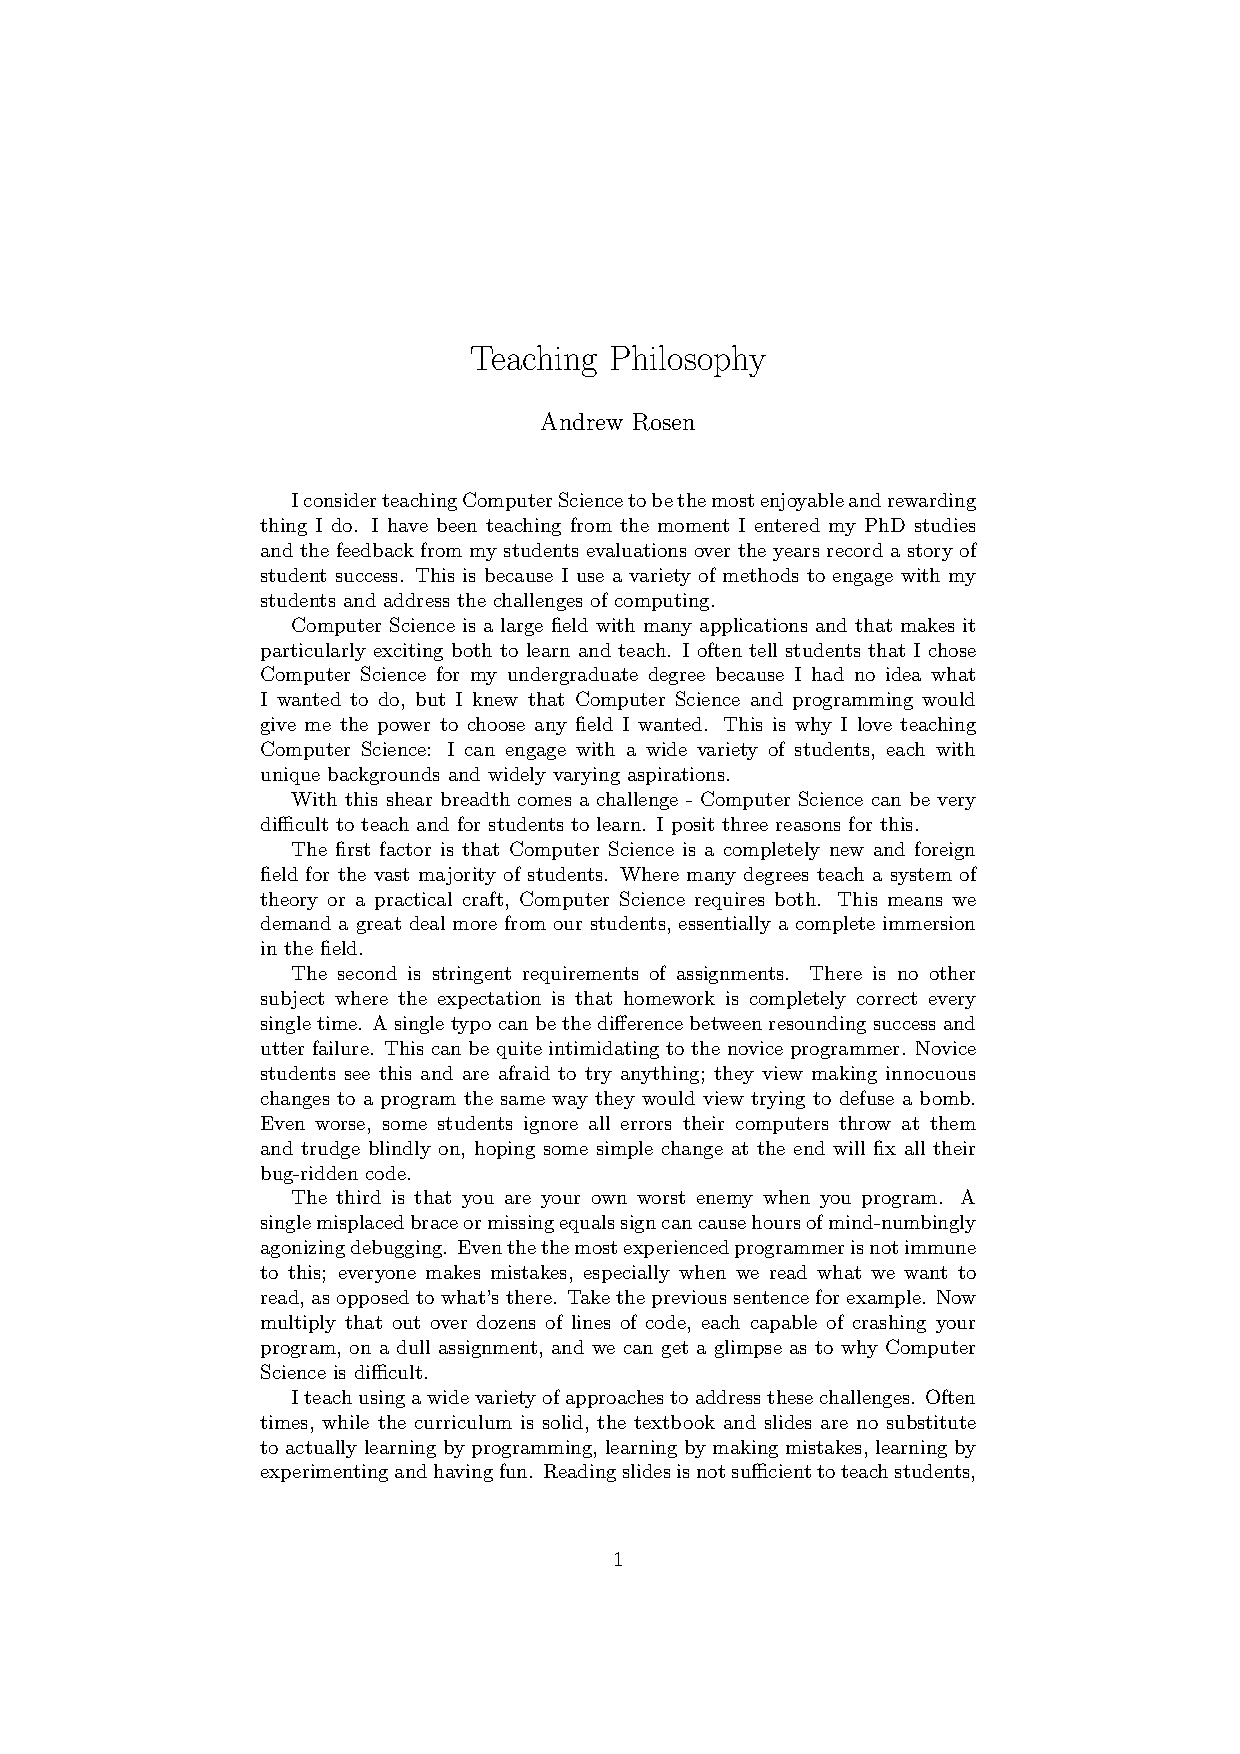
\includepdf[pages=-]{teaching.pdf}
\end{document}
